\chapter[Entraîner et évaluer]{Entraîner et évaluer un modèle}

\lettrine{A}{fin de valider} la rigueur de notre jeu de données et la pertinence de notre schéma d'annotation, l'aboutissement de ce travail réside dans la conversion de la vérité terrain en une capacité d'inférence sur des corpus inédits. C'est en effet à travers l'épreuve de l'entraînement que la modélisation conceptuelle se traduit en un outil opérationnel pour l'analyse documentaire.

Ce chapitre retrace l'ensemble du protocole expérimental, de l'entraînement à l'évaluation du modèle. Nous détaillerons d'abord la configuration des hyperparamètres, ces derniers leviers sur lesquels nous pouvons agir pour optimiser l'efficacité ou les performances du modèle. Nous analyserons ensuite les résultats obtenus à l'aune des métriques de détection, en confrontant les indicateurs statistiques aux exigences concrètes du dépouillement historique. Enfin, nous étudierons les principales erreurs de prédiction afin de dégager des pistes d'amélioration ciblées, envisageant l'évaluation non pas comme un terme définitif, mais comme le moteur d'une démarche itérative.

\section{Les hyperparamètres}

Les hyperparamètres sont les variables de configuration fixées par l'expérimentateur avant le lancement de l'entraînement. Contrairement aux paramètres (les poids et biais du réseau de neurones), qui sont appris et ajustés automatiquement par rétropropagation du gradient, les hyperparamètres pilotent la dynamique de l'apprentissage et définissent le cadre structurel dans lequel le modèle évolue.

La performance d'un algorithme de vision par ordinateur dépend de sa capacité à généraliser ses inférences sur des documents d'un type différent de ses documents d'entraînement. Cette capacité de généralisation désigne l'aptitude d'un modèle à maintenir de bonnes performances sur des images inédites, au-delà de son seul corpus d'apprentissage. À l'inverse, l'écueil principal de l'entraînement réside dans le surapprentissage (\textit{overfitting}) : le réseau mémorise alors les bruits et les spécificités propres aux données d'origine au lieu d'en extraire des caractéristiques visuelles réellement représentatives. Le contrôle de ces hyperparamètres conditionne la capacité du réseau à extraire des motifs abstraits, à gérer les variations d'échelle et à généraliser sur de nouvelles sources sans tomber dans le piège du surapprentissage.
Les hyperparamètres structurants en vision par ordinateur s'articulent autour de quatre grands axes :

\begin{description}
	\item[Dimensionnement de l'entrée et charge mémoire :]\hfill
	\begin{itemize}
		\item \textbf{Taille de l'image :} Définit la résolution spatiale des images fournies au réseau (par exemple $640 \times 640$ pixels). Une résolution élevée est essentielle pour détecter des objets de petite taille ou préserver les détails fins d'une mise en page, mais elle augmente de manière quadratique l'empreinte en mémoire VRAM et les temps de calcul.
		\item \textbf{Taille de lot (\textit{Batch Size}) :} Une taille de lot importante ($32$ ou $64$ images) permet au modèle de dégager une tendance générale très stable, puisqu'il tire ses enseignements d'un large échantillon d'un seul coup. À l'inverse, un lot réduit ($8$ ou $16$ images) oblige le modèle à s'ajuster plus fréquemment, sur la base de très peu d'exemples. Cet apprentissage, qui devient alors volontairement plus instable, peut être utilisé comme un garde-fou : il empêche la machine de s'enfermer dans de fausses déductions, par exemple, se convaincre qu'une tâche d'humidité récurrente est une illustration. Traiter les images par petits groupes force ainsi le modèle à rester adaptable face à la grande hétérogénéité matérielle des documents.
	\end{itemize}
	
	\item[Optimisation et dynamique d'apprentissage :]\hfill
	\begin{itemize}
		\item \textbf{Le taux d'apprentissage initial (\textit{Learning Rate} - $lr$) :} Il détermine l'ampleur des corrections que le modèle s'applique à lui-même lorsqu'il identifie une erreur. Un taux trop fort pousse le modèle à réagir de manière excessive (techniquement, on parle de \og divergence de la fonction de perte \/\textit{loss function}\/ \fg) ; dans les faits, le modèle n'arrive plus à stabiliser ses poids ni à progresser continuellement en raison de la trop grande volatilité de ses prédictions. À l'inverse, un taux trop faible rend le modèle excessivement timide dans ses déductions, ce qui conduit à une stagnation prématurée de son apprentissage.
		\item \textbf{La planification du taux d'apprentissage (\textit{LR Scheduler}) :} Elle adapte la cadence du modèle tout au long de son entraînement. Le réseau commence par apprendre rapidement pour dégager la structure globale des documents, puis réduit progressivement l'ampleur de ses corrections. Une volatilité élevée au début lui permet de découvrir la structure des documents, tandis qu'une volatilité basse en fin d'entraînement permet de consolider les acquis.
		\item \textbf{La décroissance des poids (\textit{Weight Decay}) :} C'est une règle de régularisation qui empêche le modèle d'accorder une importance excessive à un détail visuel isolé. En appliquant une forme d'oubli progressif sur les pondérations du réseau, cette technique évite au modèle de sur-interpréter les particularités idiosyncratiques des données d'entraînement.
	\end{itemize}
	
	\item[L'augmentation artificielle des données :]\hfill
	En vision artificielle, la quantité et la diversité des données sont déterminantes. Les hyperparamètres d'augmentation génèrent des variations artificielles des images d'origine sans coût d'annotation supplémentaire. La plupart des bibliothèques d'entraînement appliquent automatiquement des transformations géométriques (rotations, translations, cisaillement, changements d'échelle) ainsi que des modifications colorimétriques (saturation, teintes). La bibliothèque YOLO d'Ultralytics intègre en outre des transformations plus complexes, telles que la juxtaposition de plusieurs images du jeu de données ou leur superposition à différents niveaux de transparence, permettant au modèle de développer une meilleure robustesse face à une forte densité d'éléments à détecter.
	
	\item[L'équilibrage des priorités de détection (\textit{Loss Balancing}) :]\hfill
	Lors d'une tâche d'inférence, le modèle doit réussir simultanément trois missions : repérer où se trouve un élément, déterminer sa nature et ajuster ses contours. Ce paramétrage permet de pondérer les priorités de la machine afin qu'elle ne néglige aucune de ces étapes : \hfill
	\begin{itemize}
		\item \textbf{Le repérage de la zone ($\text{Box Loss } L_{\text{box}}$) :} Il évalue la capacité du modèle à placer son cadrage au bon endroit sur la page.
		\item \textbf{L'identification de la catégorie ($\text{Class Loss } L_{\text{cls}}$) :} Il contrôle si le modèle attribue l'étiquette sémantique correcte à la zone encadrée.
		\item \textbf{La précision des bordures ($\text{DFL } L_{\text{dfl}}$) :} Il s'assure de la finesse du découpage des contours. C'est la finition qui permet au cadre de coller aux limites visuelles de l'objet à détecter, même dans des cas difficiles (flou d'impression, dégradation du papier ou chevauchement de structures).
	\end{itemize}
\end{description}

L'optimisation des hyperparamètres consiste à rechercher la meilleure combinaison de réglages pour maximiser les capacités du modèle. Dans le cadre d'un projet de vision artificielle appliquée à l'analyse documentaire, l'enjeu est d'éviter le surapprentissage en maintenant une bonne capacité de généralisation, rationaliser le temps de calcul (souvent limité sur les infrastructures de recherche), et surtout adapter correctement l'algorithme au corpus. 

\section{Évaluer les résultats de l'inférence}

\subsection{Définir la méthodologie d'évaluation}

\subsubsection{L'importance du découpage du jeu de données (\textit{Data Splitting})}

La constitution d'un jeu de données repose sur la répartition des documents en trois sous-ensembles hermétiques : l'entraînement (\textit{train}), la validation (\textit{val}) et le test (\textit{test}). Le premier sert à l'ajustement direct des poids du réseau, tandis que le second permet d'évaluer la progression au fil des époques et de guider l'ajustement des hyperparamètres. Le jeu de test, quant à lui, doit être mis de côté et rester totalement inédit pour le modèle jusqu'à l'évaluation finale. Isolé de la phase de développement, il évite d'adapter implicitement la configuration du modèle aux spécificités de ce corpus d'évaluation. Cette séparation stricte constitue la seule garantie méthodologique d'une mesure objective de la capacité de généralisation de l'algorithme.

Idéalement, il faut répartir les données par manuscrit d'origine, et non par échantillonnage : si le jeu de données contient des pages issues de plusieurs documents, il faut distribuer des documents entiers entre les ensembles d'entraînement, de validation et de test, et jamais des pages individuelles d'un même document. Sinon, le modèle peut \og reconnaître \fg le style graphique, le papier ou les motifs récurrents d'un manuscrit vu en entraînement, ce qui gonfle artificiellement les scores de test. C'est cependant ce qui a été fait pour l'évaluation des modèles entraînés sur GenHisDoc, l'ayant réalisé après l'entraînement sans possibilité de corriger cette erreur faute de temps. Il faut également tenter d'éviter la présence de quasi-doublons entre le jeu de données d'entraînement et le jeu de données de test, certains sous-corpora utilisés dans GenHisDoc possédant de nombreux quasi-doublons, comme S-VED ou Horae. La définition du quasi-doublon s'avère par ailleurs très délicate à formaliser (deux images pouvant apparaître similaires à un humain alors que cela n'handicape pas l'entraînement du modèle, et inversement).

\subsubsection{La représentativité de la distribution réelle}

Idéalement, le jeu de test doit refléter les conditions d'usage réel du modèle, et non pas seulement la distribution du jeu d'entraînement :

\begin{itemize}
	\item \textbf{Diversité des sources :} prise en compte des différentes périodes historiques, des types de documents variés, ainsi que des dégradations et des défauts de numérisation.
	
	\item \textbf{Diversité des classes :} représentation suffisante de toutes les catégories d'intérêt — en veillant à la problématique de la distribution à queue longue —, un jeu de test dominé par la classe majoritaire risquant de masquer les faiblesses sur les cas minoritaires.
\end{itemize}

De surcroît, la constitution du jeu de test doit être stratifiée selon les classes, les types de documents et, de préférence, la difficulté (la densité d'objets par page). Avec un total de plus de 8\,000 images, notre jeu de test compte environ 900 images et plus de 1\,600 vérités terrain (GT), ce qui est suffisant pour garantir que l'ensemble des classes de GenHisDoc est correctement représenté.

\subsection{Résultats pour GenHisDoc}

Il s'agit de jauger le compromis fondamental entre l'exhaustivité de la recherche (le rappel) et la fiabilité des détections restituées (la précision). Pour apprécier ces performances en situation réelle, les résultats obtenus par notre modèle entraîné sur GenHisDoc sont confrontés à ceux du modèle historiquement déployé au sein de l'application AIKON, à l'aune des indicateurs statistiques détaillés dans le tableau~\ref{tab:GenHisDocYolo}.

\subsubsection{Comprendre les métriques générales}

Les résultats témoignent d'un niveau de performance élevé et homogène du modèle GenHisDoc, aussi bien sur la classe \textit{Illustration} que sur l'ensemble des classes du schéma d'annotation. Le score AP@50 atteint $87{,}87\,\%$ pour la seule classe \textit{Illustration} et se maintient à un niveau comparable ($84{,}04\,\%$) lorsque l'ensemble des classes est pris en compte, malgré un volume de vérités terrain nettement supérieur ($1\,659$ occurrences contre $558$) et, par conséquent, une tâche de discrimination plus exigeante. Cette stabilité suggère que le modèle ne doit pas sa performance à une spécialisation étroite sur un type d'objet visuel particulier, mais qu'il généralise correctement à la diversité des éléments à détecter dans les documents historiques. La précision et le rappel restent tous deux élevés et proches l'un de l'autre, tant pour la classe \textit{Illustration} ($0{,}8623$ et $0{,}8978$) que toutes classes confondues ($0{,}8473$ et $0{,}8728$), ce qui traduit un compromis équilibré entre l'exhaustivité de la détection et la fiabilité des résultats restitués, plutôt qu'une optimisation artificielle d'une métrique au détriment de l'autre. Les scores $F_1$ qui en résultent ($0{,}8797$ et $0{,}8599$ respectivement) confirment la robustesse de cet équilibre.

L'IoU moyen des détections, supérieur à $0{,}85$ dans les deux configurations et atteignant $0{,}9033$ sur la seule classe \textit{Illustration}, indique par ailleurs une excellente qualité de localisation des boîtes englobantes, et non une simple justesse de classification : les objets détectés le sont avec un niveau de précision spatiale élevé, ce qui s'avère particulièrement crucial pour des tâches avales (\textit{downstream tasks}) comme l'extraction ou le recadrage automatique d'illustrations. Enfin, si la comparaison avec le modèle AIKON historiquement en production enrichit l'analyse, la possibilité d'une évaluation strictement monoclasse (\textit{Illustration} contre \textit{Illustration}) constitue un point méthodologique notable, dans la mesure où elle permet d'isoler la contribution du nouveau modèle et du corpus GenHisDoc indépendamment de l'élargissement du périmètre ontologique.

\begin{table}[htbp]
	\centering
	\ra{1.25}
	\caption{Comparaison des résultats d'évaluation entre GenHisDoc et Aikon. GenHisDoc est un yolo 26 large entraîné sur le dataset GenHisDoc produit durant le stage. Aikon est un yolo 5 large entraîné d'abord sur les diagrammes puis finetuné pour détecter plus généralement toutes les illustrations. C'est le modèle qui équipe actuellement Aikon.}
	\begin{tabular}{lccc}
		\toprule
		& \multicolumn{2}{c}{\textbf{GenHisDoc}} & \textbf{Aikon} \\
		\cmidrule(r){2-3} \cmidrule(l){4-4}
		\textbf{Métrique / Indicateur} & \textbf{Illustration} & \textbf{Toutes classes} & \textbf{Illustration} \\
		\midrule
		\multicolumn{4}{l}{\textit{Données de test et Détection}} \\
		\hspace{1em} Fichiers traités & 876 & 876 & 876 \\
		\hspace{1em} Nombre total de GT & 558 & 1659 & 558 \\
		\hspace{1em} IoU Moyen (Détections) & 0,9033 & 0,8595 & 0,8762 \\
		\midrule
		\multicolumn{4}{l}{\textit{Performance globale}} \\
		\hspace{1em} AP@50 (mAP@50) & \textbf{ 0,8787 (87,87\%)} & 0,8404 (84,04\%) & 0,4815 (48,15\%) \\
		\midrule
		\multicolumn{4}{l}{\textit{Métriques au seuil fixe ($\ge$ 0,25)}} \\
		\hspace{1em} Vrais Positifs (TP) & 501 & 1448 & 355 \\
		\hspace{1em} Faux Positifs (FP) & 80 & 261 & 208 \\
		\hspace{1em} Faux Négatifs (FN) & 57 & 211 & 203 \\
		\hspace{1em} Précision & 0,8623 & 0,8473 & 0,6306 \\
		\hspace{1em} Rappel (Recall) & 0,8978 & 0,8728 & 0,6362 \\
		\hspace{1em} Score F1 & \textbf{0,8797} & 0,8599 & 0,6334 \\
		\bottomrule
	\end{tabular}
	\label{tab:GenHisDocYolo}
\end{table}
\subsubsection{Comprendre les métriques par classes}

\begin{figure}[h]
	\centering
	\begin{subfigure}{0.48\textwidth}
		\centering
		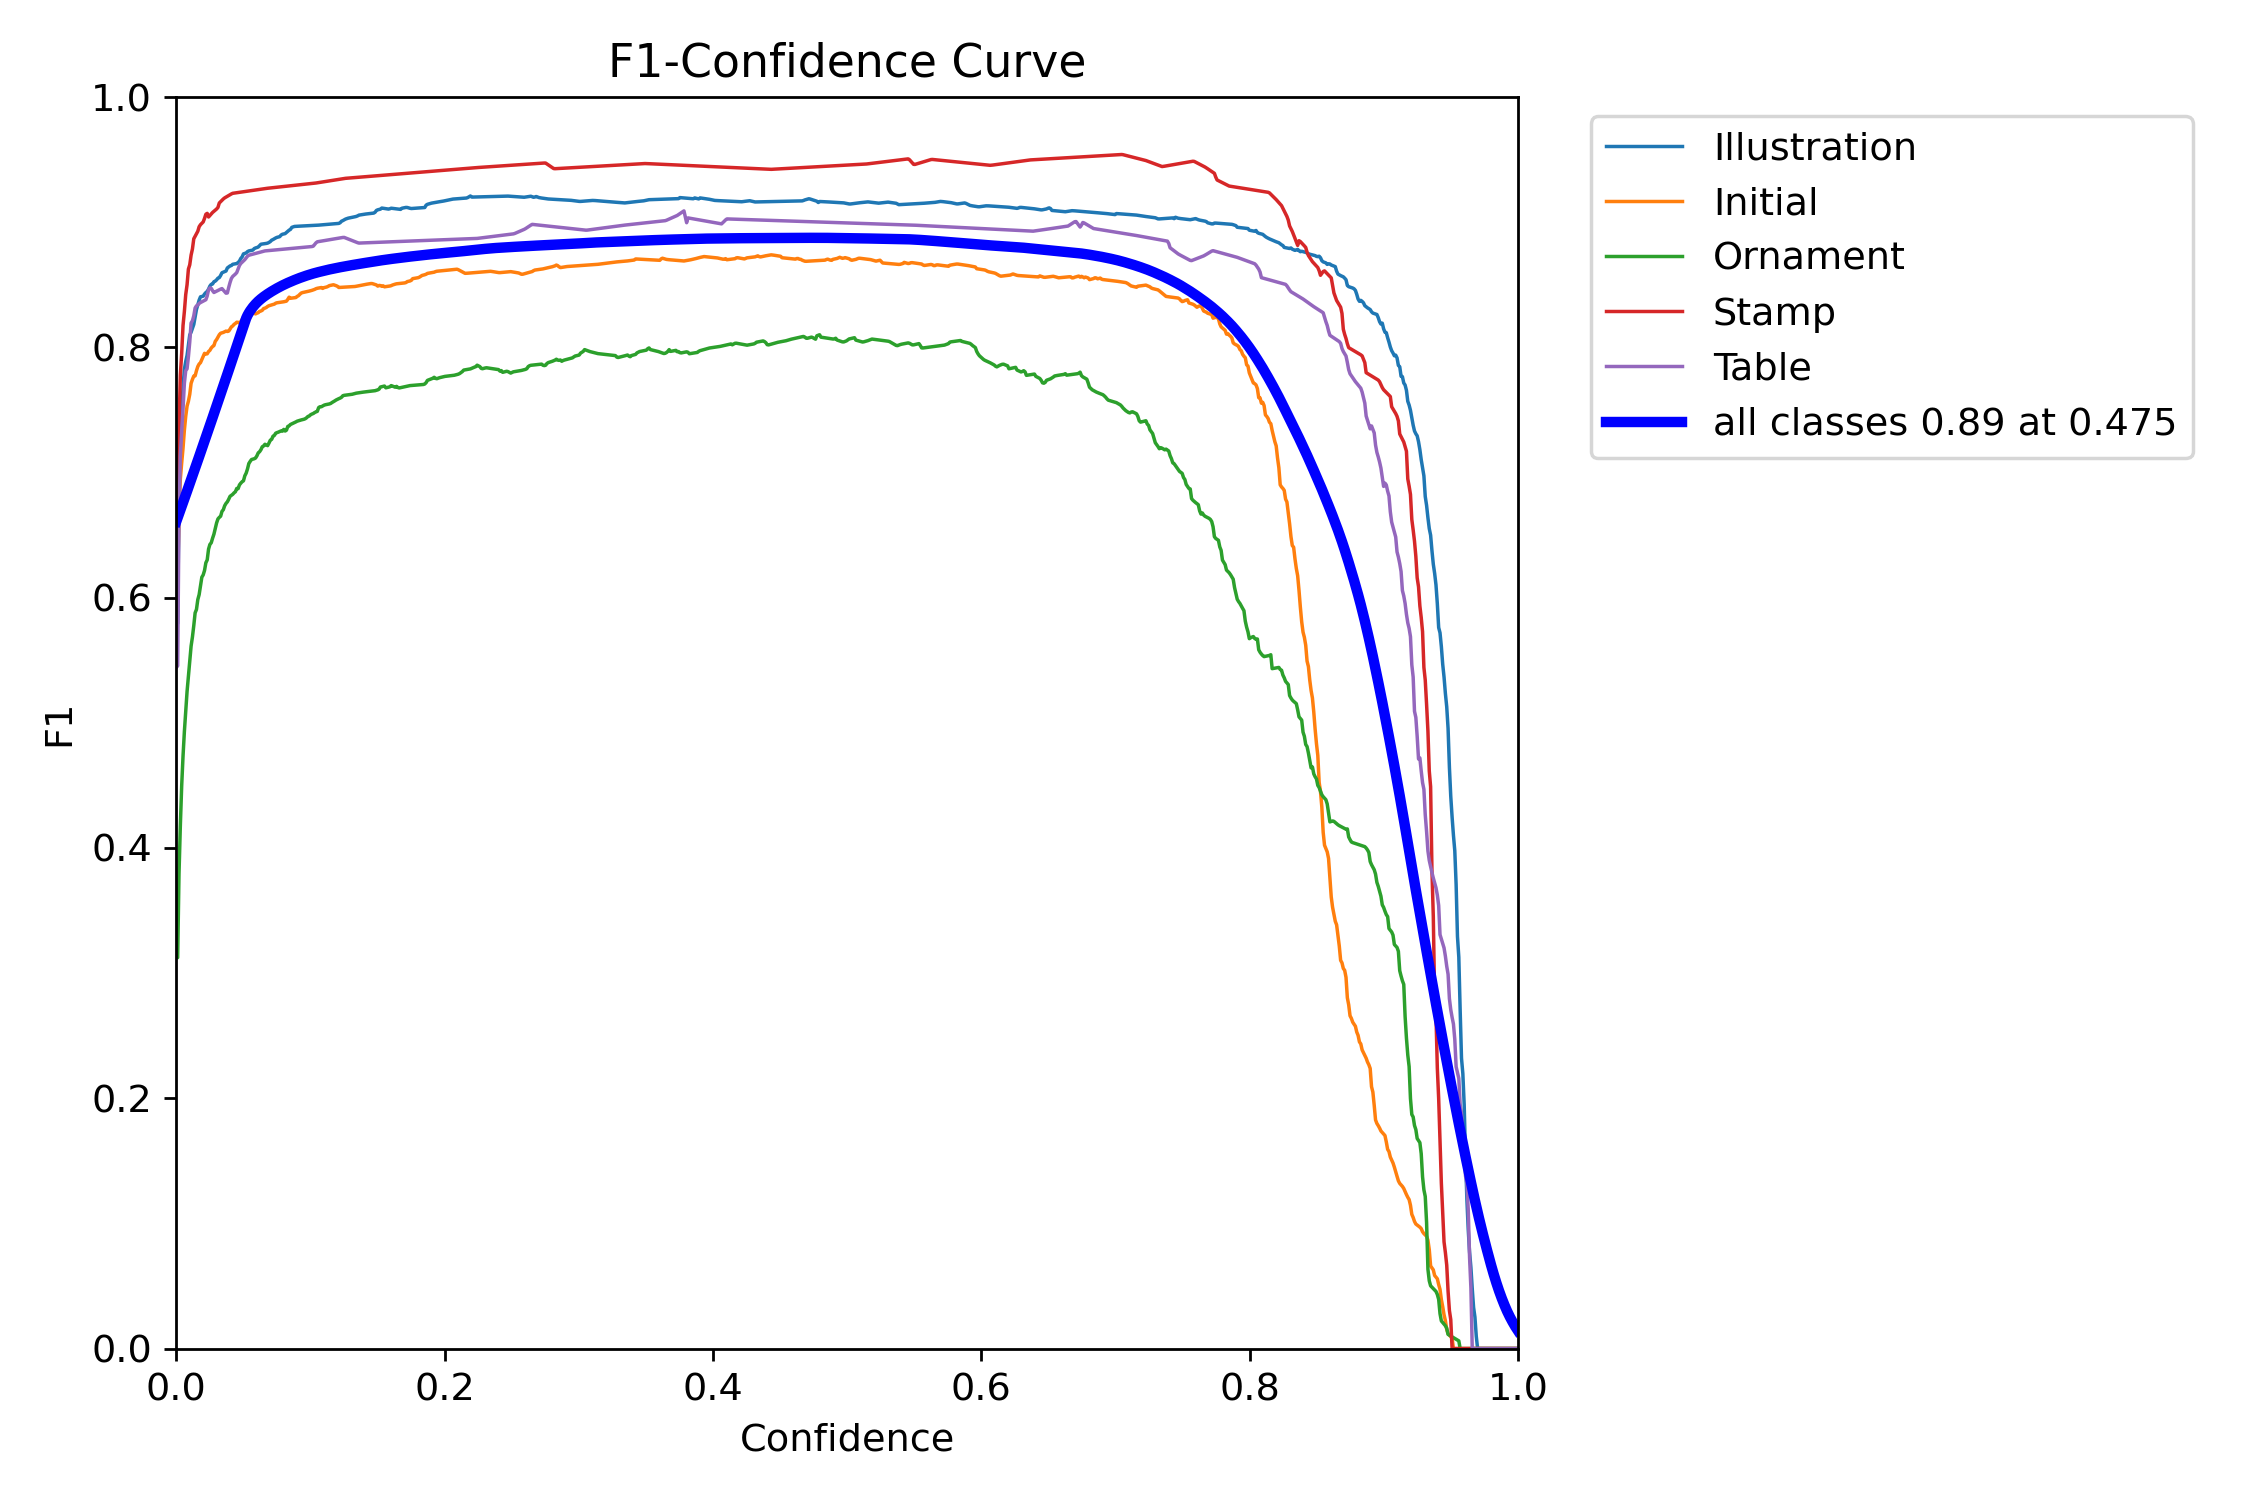
\includegraphics[width=\linewidth, height=8cm, keepaspectratio]{img/BoxF1_curve.png}
		\caption{Score $F_1$}
		\label{fig:f1score}
	\end{subfigure}
	\hfill
	\begin{subfigure}{0.48\textwidth}
		\centering
		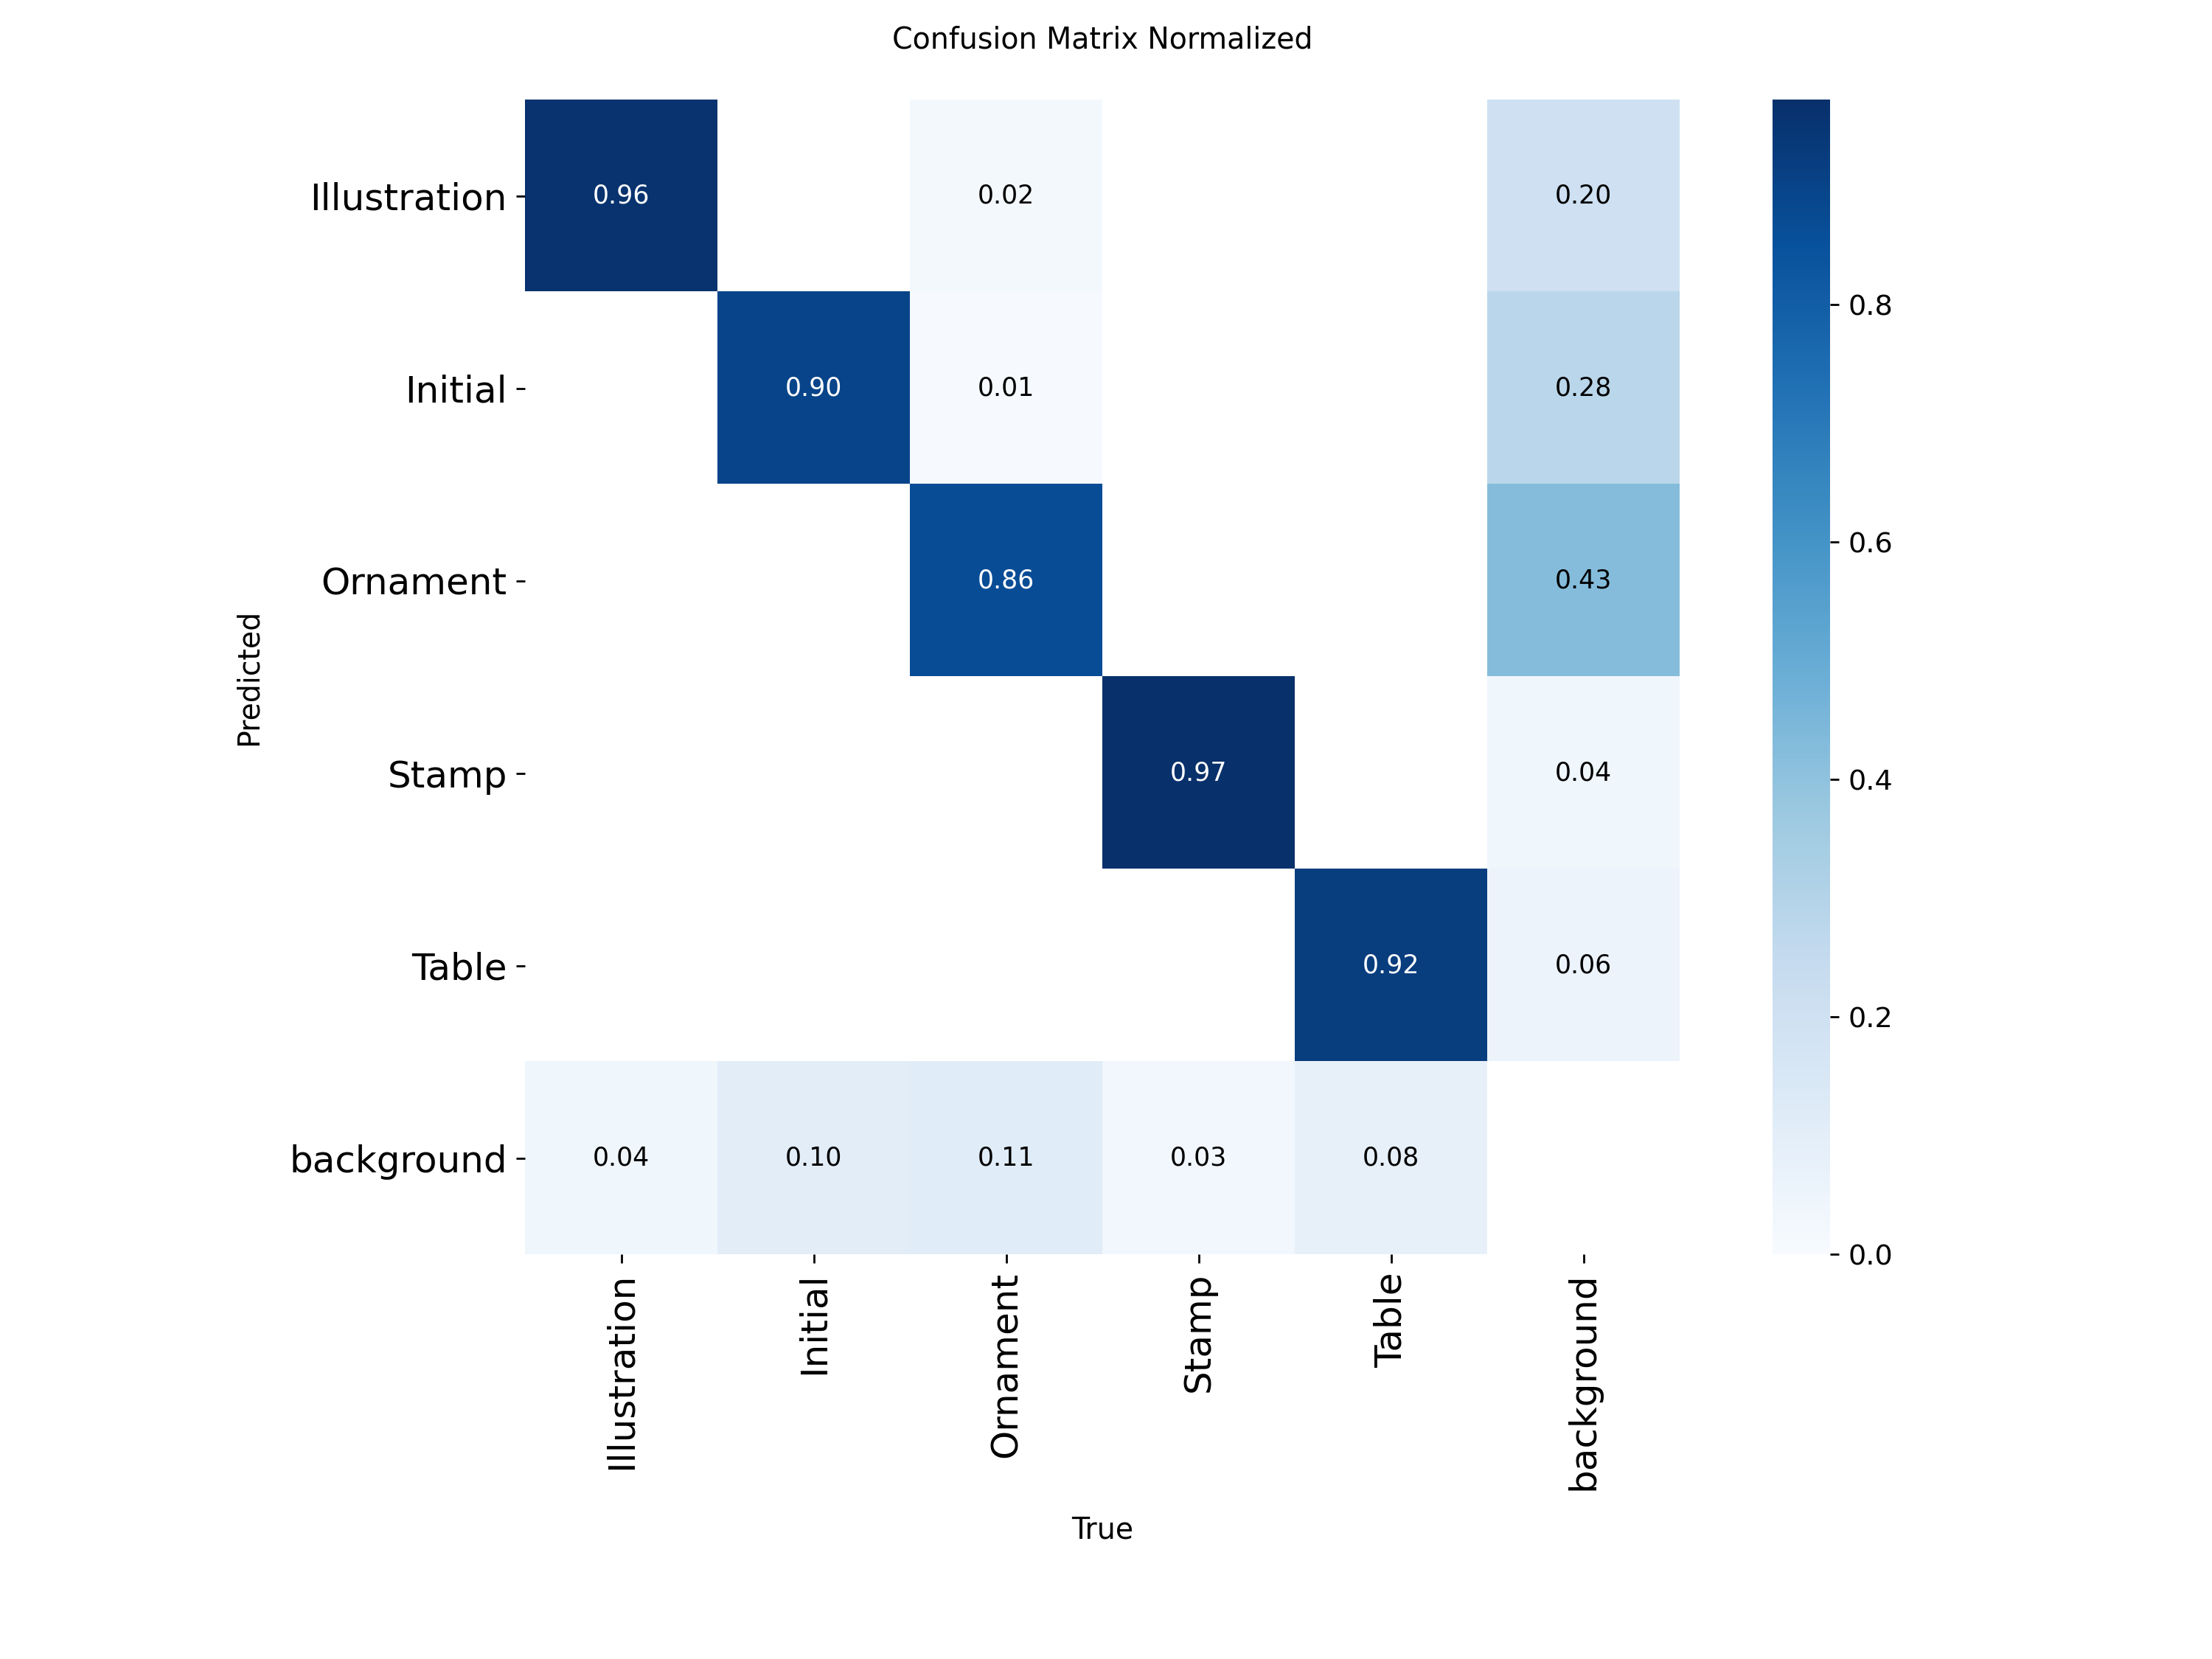
\includegraphics[width=\linewidth, height=8cm, keepaspectratio]{img/confusion_matrix_normalized.png}
		\caption{Matrice de confusion normalisée}
		\label{fig:confusionmatrix}
	\end{subfigure}
	\caption{Représentation des scores $F_1$ et de la matrice de confusion normalisée des classes du modèle entraîné sur GenHisDoc.}
	\label{fig:confusionF1}
\end{figure}

{\raggedright\textbf{Le score $F_1$ par classes :}}
\begin{itemize}
	\item \textbf{\textit{Stamp}} (en rouge) est la classe la plus performante, affichant un plateau proche de $0{,}95$ sur une plage de confiance très large (jusqu'à environ $0{,}7$). Ce résultat s'explique par la nature de l'objet, visuellement homogène et hautement discriminant (formes géométriques régulières et contrastes marqués).
	
	\item \textbf{\textit{Illustration}} (en bleu) et \textbf{\textit{Table}} (en violet) se comportent de manière satisfaisante, avec des scores oscillant entre $0{,}88$ et $0{,}92$, en adéquation avec l'agrégat global. L'efficacité de la détection des tableaux constitue l'une des surprises notables de ce travail : alors que cette classe pouvait initialement paraître difficile à circonscrire en raison de sa variabilité typographique, l'homogénéité des principes d'annotation a permis au modèle de la modéliser avec succès.
	
	\item \textbf{\textit{Initial}} (en orange) se situe en retrait, autour de $0{,}85\text{--}0{,}87$, avec un déclin de performance qui s'amorce plus précocement (vers $0{,}6$ de confiance) que pour les autres catégories. Le modèle manifeste ici une moindre certitude, imputable soit à une forte hétérogénéité visuelle (les lettrines historiques adoptant des styles extrêmement variés), soit à des imprécisions dans les consignes d'annotation, soit encore à la présence d'éléments parasites morphologiquement proches, tels que les pieds-de-mouche (\textit{pilcrows}, $\P$).
	
	\item \textbf{\textit{Ornament}} (en vert) constitue la classe la plus fragile, plafonnant à environ $0{,}80$ avec une décroissance marquée dès $0{,}5\text{--}0{,}6$ de confiance. Cette faiblesse témoigne de la difficulté inhérente à la détection de cette catégorie, caractérisée par une forte variabilité intra-classe (les ornements typographiques et encadrements historiques revêtant des formes d'une grande hétérogénéité).
\end{itemize}

{\raggedright\textbf{La matrice de confusion normalisée :}}

Chaque colonne correspond à une classe réelle (\textit{True}) et répartit le devenir de tous les objets réels de cette catégorie entre les différentes prédictions possibles. La ligne \og \textit{background} \fg, située en bas, indique la proportion d'objets réels manqués (faux négatifs, prédits comme une absence d'objet). La colonne \og \textit{background} \fg, située à droite, fonctionne différemment : elle répartit l'ensemble des fausses détections (prédictions sans objet réel correspondant, ou faux positifs) entre les classes prédites à tort.

\begin{table}[h]
	\centering
	\ra{1.25}
	\begin{tabular}{lcc}
		\toprule
		\textbf{Classe} & \textbf{Bien détecté} & \textbf{Manqué} ($\text{FN} \to \text{Background}$) \\
		\midrule
		\textit{Stamp} & $0{,}97$ & $0{,}03$ \\
		\textit{Illustration} & $0{,}96$ & $0{,}04$ \\
		\textit{Table} & $0{,}92$ & $0{,}08$ \\
		\textit{Initial} & $0{,}90$ & $0{,}10$ \\
		\textbf{\textit{Ornament}} & \textbf{0{,}86} & \textbf{0{,}11 (+ 0{,}03 mal classé)} \\
		\bottomrule
	\end{tabular}
	\caption{Extraction des taux de détection et des faux négatifs par classe issus de la matrice de confusion normalisée.}
	\label{tab:matrice}
\end{table}

La classe \textit{Ornament} s'avère bien la plus fragile, affichant le taux de rappel le plus faible et se révélant être la seule à présenter des confusions inter-classes non négligeables : $2\,\%$ des \textit{Ornament} réels sont prédits à tort comme des illustrations, et $1\,\%$ comme des lettrines. Cette porosité est cohérente d'un point de vue codicologique, les ornements typographiques et encadrements se rapprochant parfois visuellement de motifs décoratifs d'illustrations ou de lettrines historiées, ce qui complexifie leur distinction par le modèle.

Nous avions également ajouté un système de découpage des lettrines trop complexes, dissociant l'espace de la lettre, considéré comme une lettrine, et l'espace de son ornementation, considéré comme un ornement. Ce système, hérité du corpus Horae, permet de limiter le bruit pour les lettrines immenses qui occupent la moitié d'une page.

L'analyse de la matrice de confusion révèle en outre que la classe \textit{Ornament} concentre à elle seule $43\,\%$ de l'ensemble des fausses détections du modèle (contre $28\,\%$ pour \textit{Initial}, $20\,\%$ pour \textit{Illustration}, $6\,\%$ pour \textit{Table} et seulement $4\,\%$ pour \textit{Stamp}). Autrement dit, lorsque le modèle \og hallucine \fg{} un objet inexistant, il s'agit le plus souvent d'un ornement.

\section{Les pistes d'amélioration}

Les premiers résultats obtenus sur GenHisDoc, aussi encourageants soient-ils dans l'ensemble, mettent en évidence certaines limites qu'il convient d'interroger avant d'envisager une simple poursuite de l'entraînement. Nous devons reconsidérer en partie, au-delà du seul réglage technique du modèle, la pertinence des choix méthodologiques opérés en amont, qu'il s'agisse de la constitution du corpus, de la définition des classes, ou de l'adéquation de l'approche retenue avec les besoins spécifiques de l'analyse de documents historiques. C'est cette mise en tension entre les résultats observés et les choix initiaux qui doit guider la définition des axes d'amélioration à privilégier.

Nous détaillons dans cette section les différentes approches testées ainsi que leurs résultats respectifs.

\subsection{Modifier les hyperparamètres}

Le réglage des hyperparamètres constitue le levier d'amélioration le plus immédiat, dans la mesure où il n'implique de revenir ni sur les annotations ni sur la définition des classes : il s'agit d'optimiser la manière dont le modèle apprend. Cet axe est aussi celui pour lequel les courbes de perte et de convergence, déjà présentées, offrent le diagnostic le plus direct, en révélant d'éventuels signes de sous-apprentissage, de surapprentissage ou une durée d'entraînement mal calibrée.

Les modèles que nous avons entraînés sur GenHisDoc obéissaient tous aux mêmes hyperparamètres ($640 \times 640$ pixels en taille d'image, $100$ époques d'entraînement, paramètres par défaut pour le reste des hyperparamètres).

L'examen conjoint des pertes d'entraînement et de validation (figure~\ref{fig:losses}) constitue le point le plus instructif du point de vue du réglage des hyperparamètres. Si les deux courbes décroissent de concert jusqu'aux alentours de l'époque $60$, un écart croissant apparaît ensuite entre la perte de classification d'entraînement, qui continue de chuter fortement, et son homologue de validation, qui se stabilise puis stagne autour de $0{,}5$ à partir de l'époque $70$ : ce découplage constitue un indice classique de début de surapprentissage, contenu néanmoins par le fait que les métriques de validation (précision, rappel, $\text{mAP}_{50}$, $\text{mAP}_{50\text{--}95}$) n'accusent pas de dégradation correspondante et se maintiennent sur un plateau élevé entre les époques $70$ et $100$. Le plateau atteint dès l'époque $70$ pour la $\text{mAP}_{50}$ ($\approx 0{,}91$) et la poursuite d'une lente progression de la $\text{mAP}_{50\text{--}95}$ (de $0{,}69$ à $0{,}70$) jusqu'aux époques $72\text{--}83$ indiquent que la durée d'entraînement de $100$ époques était globalement bien calibrée, sans marge de progression significative résiduelle, et qu'un arrêt anticipé (\textit{early stopping}) autour des époques $70\text{--}80$ aurait vraisemblablement permis d'obtenir des performances quasi identiques à un coût de calcul moindre.

\begin{figure}[h]
	\centering
	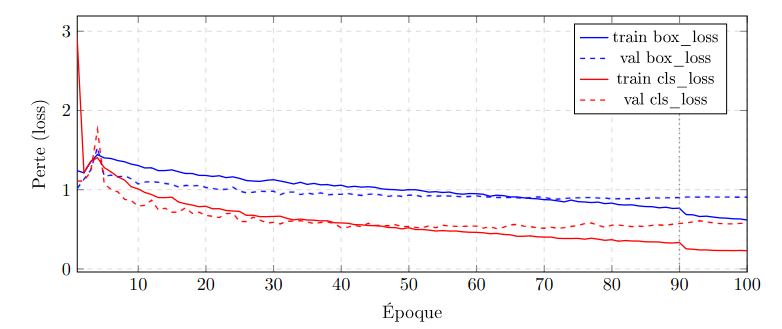
\includegraphics[width=0.8\textwidth]{img/loss.png}
	\caption{Comparaison des pertes d'entraînement et de validation (\textit{box loss} et \textit{classification loss}).}
	\label{fig:losses}
\end{figure}

\subsection{Mettre en place une meilleure méthodologie d'évaluation}

La pertinence des indicateurs statistiques présentés précédemment dépend directement de la rigueur avec laquelle le jeu de données d'évaluation est constitué.

Corriger les biais méthodologiques identifiés précédemment afin d'obtenir un jeu de test et de validation parfaitement sain constitue un enjeu majeur pour l'évolution du projet. Un découpage strict, opéré par manuscrits distincts et expurgé de tout quasi-doublon, permet d'abord d'obtenir des métriques beaucoup plus fidèles et réalistes quant aux performances de l'algorithme en conditions réelles de dépouillement. L'analyse de ces erreurs, désormais affranchie de toute fuite de données, fournit en aval des informations précieuses pour cibler les corrections à apporter (ajustement de l'ontologie, ajout de documents spécifiques pour combler un manque, modification des hyperparamètres). L'évaluation ne s'apparente plus alors à un simple constat, mais devient un véritable levier d'amélioration continue.

\subsection{Modifier et faire évoluer les annotations}

Modifier et enrichir les données au sein d'un corpus d'apprentissage constitue souvent le levier le plus déterminant pour faire progresser les performances d'un modèle de vision. C'est toutefois l'un des plus coûteux en temps et en ressources humaines, puisqu'il implique de revenir sur des phases d'annotation manuelle.

\begin{description}
	\item[La correction et la purification des annotations :] Un examen qualitatif des prédictions erronées peut révéler une insuffisance de la vérité terrain. Par exemple, dans le cas de GenHisDoc, reprendre les annotations de la classe \textit{Ornament} pour les préciser géométriquement et les corriger ontologiquement permettrait d'améliorer les performances du modèle.
	
	\item[Changer les directives d'annotation (\textit{guidelines}) :] Conserver les mêmes classes tout en précisant la manière dont les documents doivent être découpés. En uniformisant ces consignes de saisie, on réduit drastiquement la variabilité intra-classe. Le modèle bénéficie alors d'une plus grande cohérence géométrique dans ses exemples, ce qui améliore directement sa capacité à bien dimensionner ses cadres.
	
	\item[Améliorer la représentativité des classes :] Ce problème ne concerne pas directement GenHisDoc (où les volumes d'annotations suffisent à garantir un bon équilibre), mais remédier aux déséquilibres dans la distribution des classes peut avoir un effet très bénéfique sur l'entraînement d'un modèle de vision.
\end{description}

\subsection{Transformer l'ontologie}

Cette dernière solution est la plus coûteuse, car elle revient à jeter une grande partie du travail d'annotation produit, à remanier en profondeur la vérité terrain et à reprendre l'ensemble des directives d'annotation.

\begin{description}
	\item[La simplification par fusion (regroupement) :] C'est l'approche la moins destructrice pour le jeu de données. Si l'objectif final se limite à l'extraction de zones décorées, fusionner \textit{Ornament} et \textit{Illustration} en une méta-classe supprimerait mécaniquement la confusion inter-classes et ferait chuter le taux de faux positifs. Les annotations existantes sont conservées et l'on modifie seulement leur étiquette, mais au détriment de la granularité de l'analyse historique.
	
	\item[La complexification par scission (sous-spécialisation) :] À l'inverse, si l'on exige une plus grande finesse d'analyse, il convient de scinder les catégories confondues en remplaçant \textit{Ornament} par des classes visuellement plus homogènes. Le coût est ici maximal : cette approche oblige l'équipe de recherche à rouvrir des milliers de documents annotés pour reclasser, redessiner ou redéfinir les boîtes englobantes selon de nouveaux critères.
\end{description}

Dans le cadre de GenHisDoc, l'une des modifications d'ontologie pertinentes pour améliorer l'efficacité du modèle sur les ornementations consisterait peut-être à séparer les éléments manuscrits des éléments imprimés. Si l'on souhaite à terme réintégrer des corpus de presse ou des imprimés anciens au sein de GenHisDoc, une refonte encore plus profonde de l'ontologie utilisée devrait être envisagée.